\section{Langkah-Langkah Percobaan}
\subsection{Persiapan Alat dan Bahan}
Sebelum memulai praktikum ini, praktikan mempersiapkan beberapa alat dan bahan yang diperlukan. Alat dan bahan yang praktikan bawa sendiri diantaranya, laptop yang sudah terinstall Winbox, dan kabel UTP. Sedangkan alat dan bahan yang telah disediakan adalah 2 set router mikrotik. Pengambilan dilakukan oleh perwakilan kelompok.

\subsection{Routing Statis IPv6}
\begin{enumerate}
  \item Mereset Konfigurasi Router \\
  Sebelum memulai praktikum, praktikan mereset seluruh konfigurasi pada router. Praktikan pertama-tama membuka winbox dan login ke jaringan router. Kemudian, memilih menu system > reset configuration.
  \item Mengkonfigurasi Router \\
  Setelah mereset konfigurasi, praktikan akan mengkonfigurasi ulang. Router akan dikonfigurasi agar memiliki alamat IPv6. Untuk melakukannya, praktikan membuka menu IPv6 > Addresses. Praktikan kemudian memberikan alamat sesuai modul untuk semua interface, baik yang terhubung ke laptop maupun yang terhubung dengan router lainnya. Hasil konfigurasi dapat dilihat pada gambar \ref{fig:langkaha2}.
  \item Routing Statis \\
  Setelah semua interface memiliki almat IPv6, praktikan menambahkan routing table. Untuk melakukannya, praktikan membuka menu IPv6 > Routes. Praktikan kemudia menambahkan routing pada router A dengan network address dan gateway untuk laptop B. Sedangkan pada router B, praktikan menambahkan network address dan gateway untuk laptop A. Hasil Routing Table dapat dilihat di gambar \ref{fig:langkaha3}.
  \item Mengkonfigurasi Laptop\\
  Praktikan juga mengkonfigurasi IPv6 statis untuk laptop. Praktikan membuka menu Network > IP Setting > IPv6. Kemudian emnambahkan alamta sesuai modul untuk laptop A dan laptop B.
  \item Menguji Konektivitas \\
  Setelah semuanya dikonfigurasikan, praktikan menguji koneksi dengan ping ke interface router A, router B, dan laptop lainnya. Hasil dari ping dapat dilihat pada gambar \ref{fig:langkaha5}.
\end{enumerate}

\subsection{Routing Dinamis IPv6}
\begin{enumerate}
  \item Mengkonfigurasikan Router dan Laptop \\
  Pada percobaan kedua ini, praktikan perlu untuk mengkonfigurasi kembali alamat IPv6 router dan laptop. Namun, karena alamat yang digunakan sama dengan percobaan pertama, praktikan tidak mengubahnya.
  \item Menambahkan OSPFv3 Instance dan Area \\
  Untuk melakukan routing dinamis, praktikan perlu menambahkan OSPFv3 instance. Pertama-tama, praktikan masuk ke menu Routing > OSPFv3 kemudian tab instance. Pada tab ini, praktikan menambahkan instance degan nama dan router id sesuai arahan modul. Setelah itu, praktikan membuka tab Areas pada menu yang sama dan menambahkan area sesuai arahan modul. Hasil instance dan area dapat dilihat pada gambar \ref{fig:langkahb2a} dan \ref{fig:langkahb2b}.
  \item Menambahkan Interface OSPFv3 \\
  Kemudian, agar routing bisa dilakukan dinamis antara interface router yang terhubung, praktikan menambhakan interfaces OSPFv3. Sesuai arahan modul, praktikan menambahkan konfigurasi interface, intance, dan area. Hasil seperti pada gambar \ref{fig:langkahb3}.
  \item Mengecek Neighbour dan Routing \\
  Praktikan memastikan apakah interface dari masing-masing router dapat mebaca atau mendeteksi keberadaan satu sama lain. Untuk melakukannya, praktikan memilih tab Neighbour seperti yang terlihat pada gambar \ref{fig:langkahb4}.
  \item Menguji Konektivitas \\
  Setelah semuanya dikonfigurasikan, praktikan menguji koneksi dengan ping ke interface router A, router B, dan laptop lainnya. Hasil dari ping berhasil seperti terlihat di gambar \ref{fig:langkahb5}.
\end{enumerate}

\section{Analisis Hasil Percobaan}
Percobaan pertama routing statis IPv6 bertujuan untuk memahami penggunaan IPv6 serta memahami implementasi routing pada IPv6. Kelompok praktikan berhasil mengkonfigurasi alamat iPv6 tanpa kendala baik di router maupun laptop. Sebagaimana teori bahwa IPv6 memiliki panjangan alamat 128 bit dengan format 8 kelompok hexadecimal 16 bit. Namun, format ini dapat dipersingkat dengan omiting 0000 menggunakan ::. Sehingga, praktikan tidak memasukkan full tapi hanya 2001:db8:1::1/64 yang aslinya 2001:0db8:0001:0000:0000:0000:0000:0001/64. Terdapat poin yang menarik untuk dibahas di sini, yaitu penggunaan subnet /64. IPv6 terlihat menggunakan subnet dengan ukuran yang sangat besar, jika pada standar IPv4. Namun, ternyata penggunaan subnet ini bukanlah masalah karena IPv6 memang bukan didesain untuk hemat, tetapi untuk kemudahan. suBNET /64 Iini akan digunakan pada berbagai protokol seperti SLAAC dan lain sebagainya. Yang berbeda dari IPv6 dari IPv4 ketika setting address adalah adanya address otomatis local Ipv6. Sesuai teori, address ini sangat penting untuk komunikasi dasar seperti NDP, SLAAC dan ARP. Ketika praktikum, kelompok praktikan sempat tidak sengaja mengahpus local address ini yang menyebabkan kegagalan koneksi, baik ke sesama jaringan maupun jaringan lain. Percobaan kedua routing dinamis menggunakan OSPFv3. Penggunaan OSPFv3 karena protokol ini merupakan yang paling sering digunakan untuk jaringan menengah dan besar. Protokol ini menggunakan algoritma shortest path Djikstra sehingga membutuhkan identifikasi masing-masing interface atau router untuk membuat peta topologi yang disebut SPF Tree. Selain itu, network harus dibagi menjadi area. Semua router dalam area memiliki informasi topologi yang sama dan LSDB nya sendiri. Penentuan area ini penting untuk mengurangi beban kerja router karena router hanya perlu mengetahui informasi areanya sendiri. pada percobaan ini, praktikan juga melakukan pengecekan neighbour. Dengan adanya neighbour yang terdeteksi, artinya kedua jaringan telah meenyetujui hello packet sehingga dapat berkomunikasi satu sama lain. Kelompok praktikan, sempat tidak mendapatkan neighbour ini, sehingga tidak bisa melakukan komunikasi.

\section{Hasil Tugas Modul}
Simulasikan Konfigurasi Praktikum P2 di atas mengenai Routing Dinamis dan Statis IPV6 menggunakan GNS3. \\

Berikut ini merupakan hasil simulasi menggunakan Cisco Packet Tracer. Hasil simulasi juga dpat dilihat pada file P3.pkt.

\begin{figure}[h!] 
    \centering
    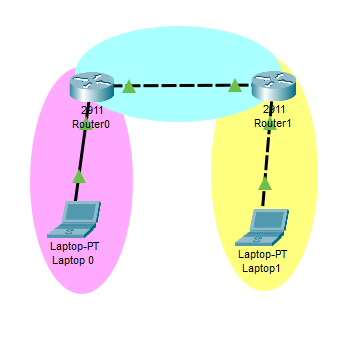
\includegraphics[width=0.5\textwidth]{tumod/simulasi.png} 
    \caption{Hasil Simulasi di Cisco Packet Tracer} 
    \label{fig:tumod1} 
\end{figure}

\subsection{Routing Statis}

\begin{figure}[H] 
    \centering
    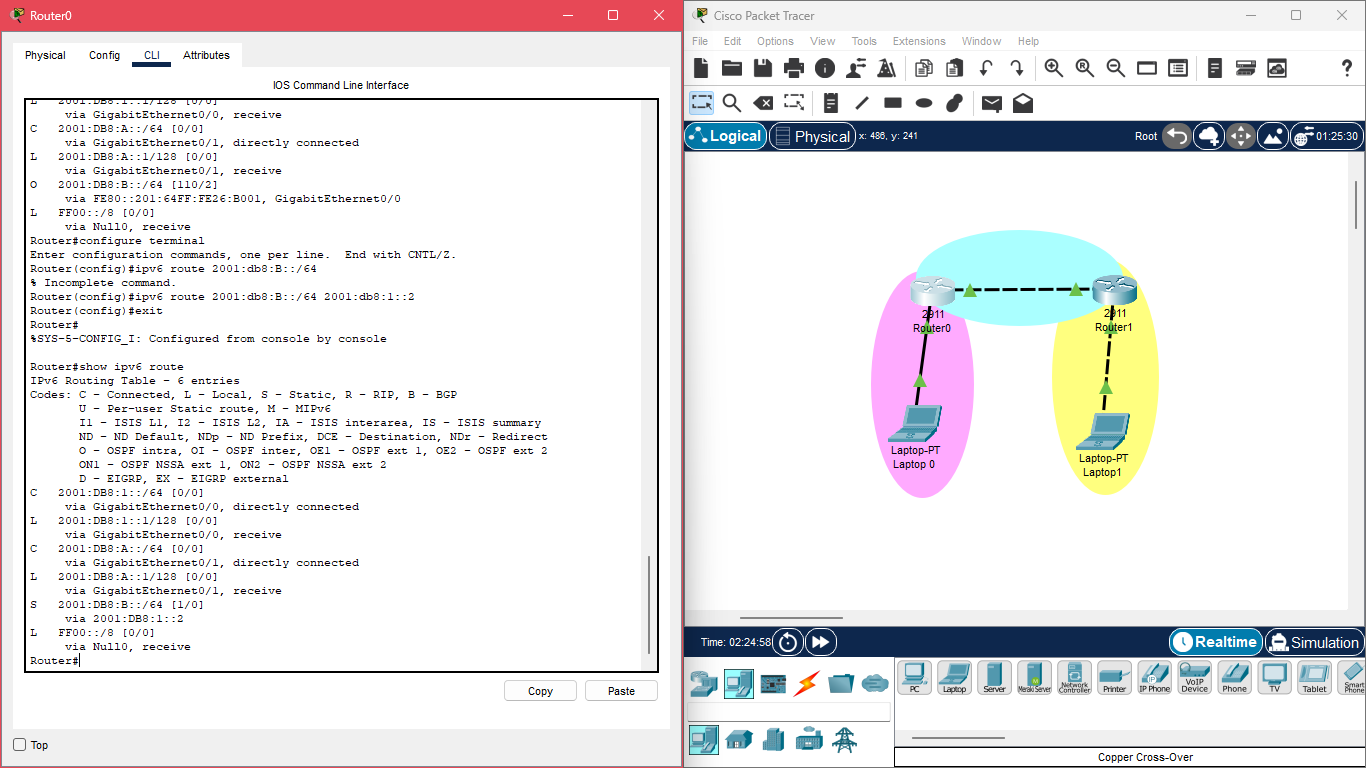
\includegraphics[width=0.5\textwidth]{tumod/jarkom tumod 5.png} 
    \caption{Setting Routing di Router A} 
    \label{fig:tumod4} 
\end{figure}

\begin{figure}[H] 
    \centering
    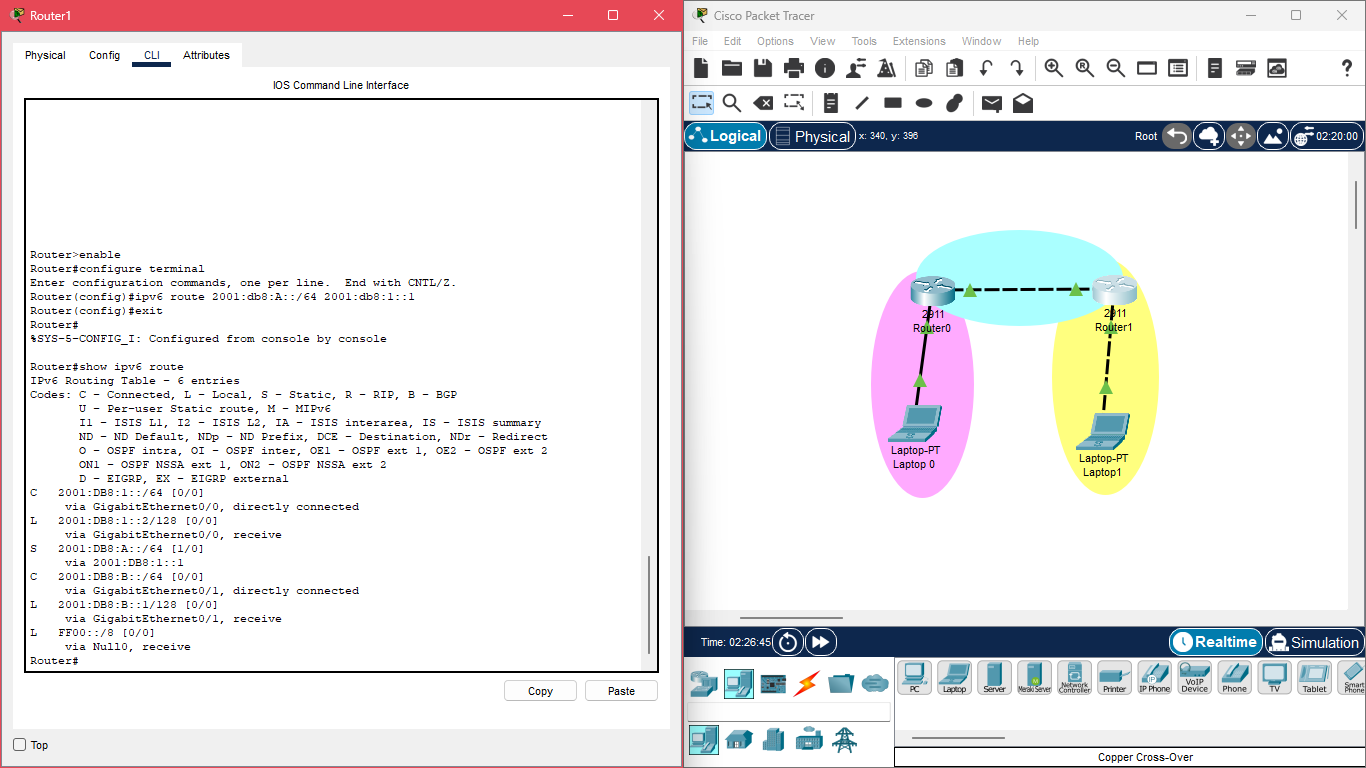
\includegraphics[width=0.5\textwidth]{tumod/jarkom tumod 6.png} 
    \caption{Setting Routing di Router B} 
    \label{fig:tumod5} 
\end{figure}

\begin{figure}[H] 
    \centering
    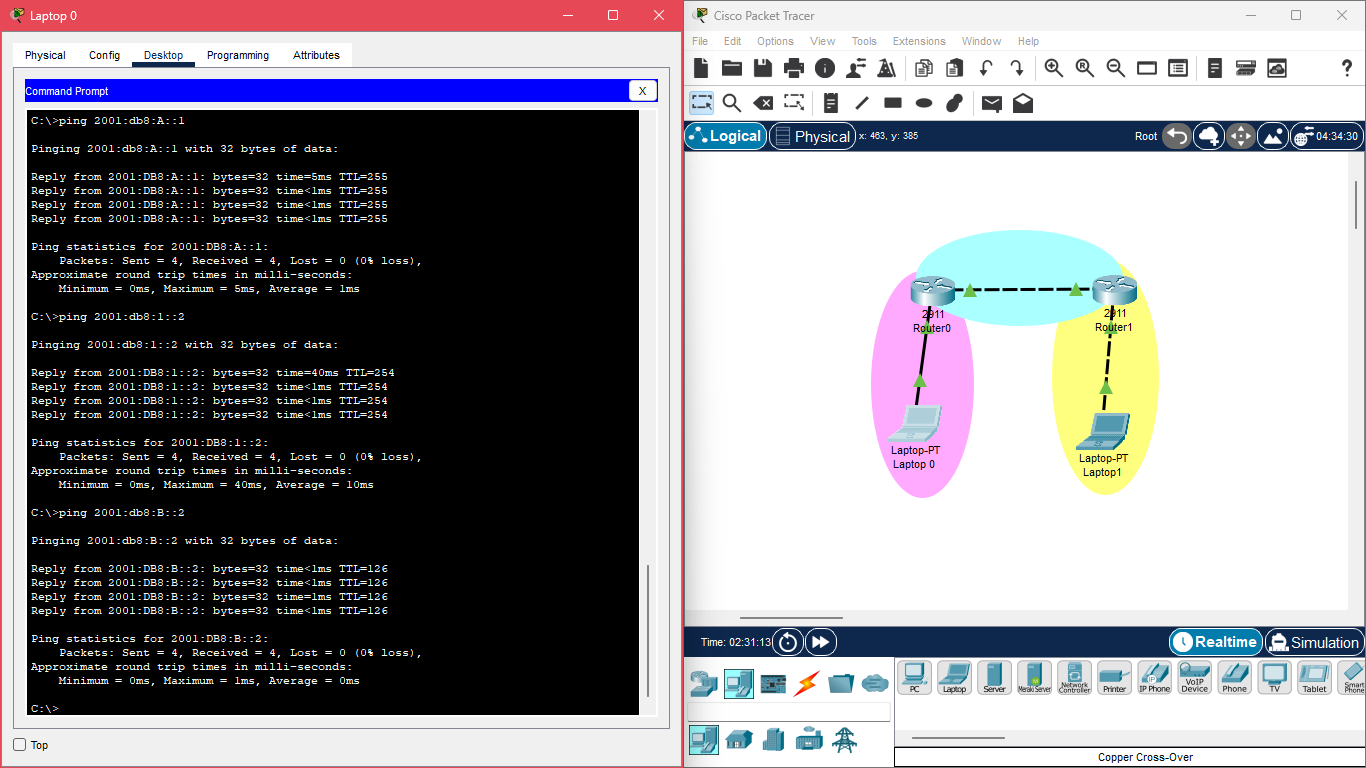
\includegraphics[width=0.5\textwidth]{tumod/jarkom tumod 7.png} 
    \caption{Hasil Ping pada Laptop A} 
    \label{fig:tumod6} 
\end{figure}

\begin{figure}[H] 
    \centering
    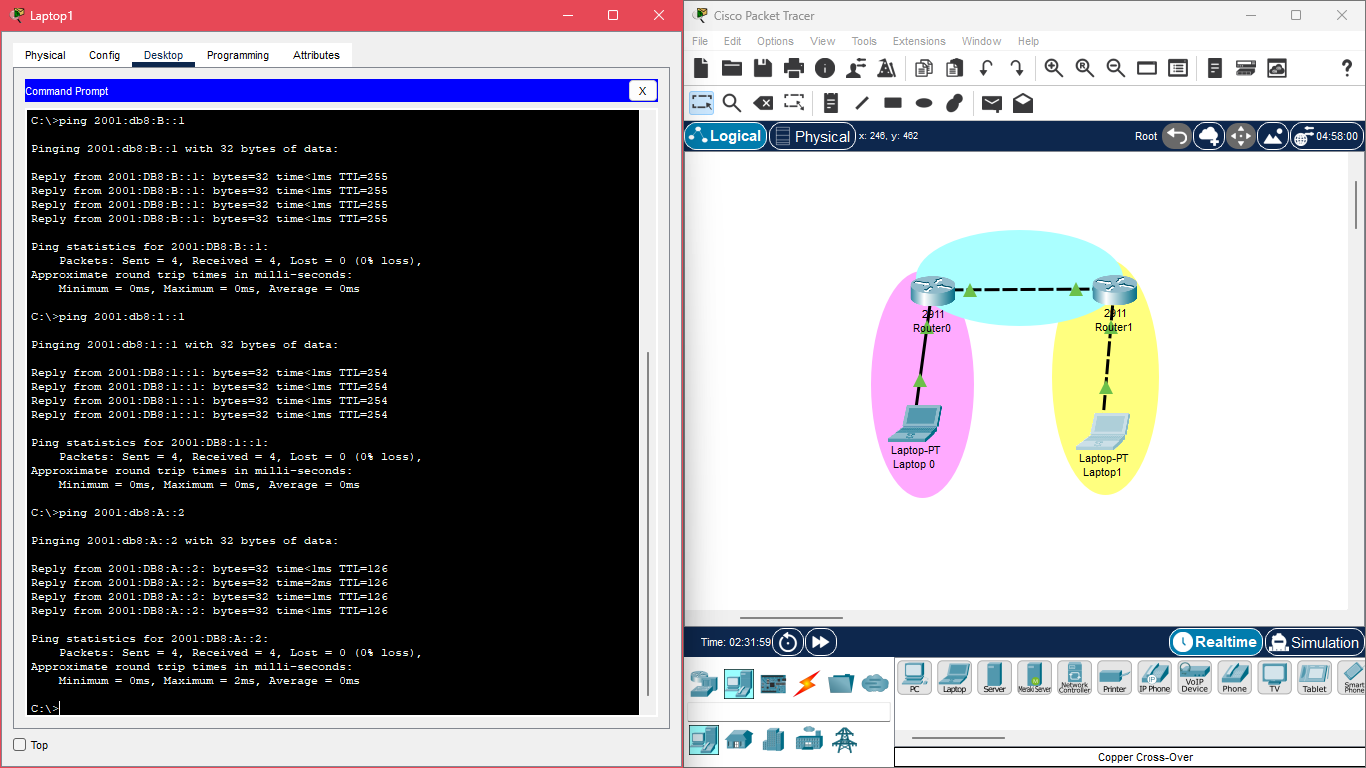
\includegraphics[width=0.5\textwidth]{tumod/jarkom tumod 8.png} 
    \caption{Hasil Ping pada Laptop B} 
    \label{fig:tumod7} 
\end{figure}

\subsection{Routing OSPFv3}

\begin{figure}[H] 
    \centering
    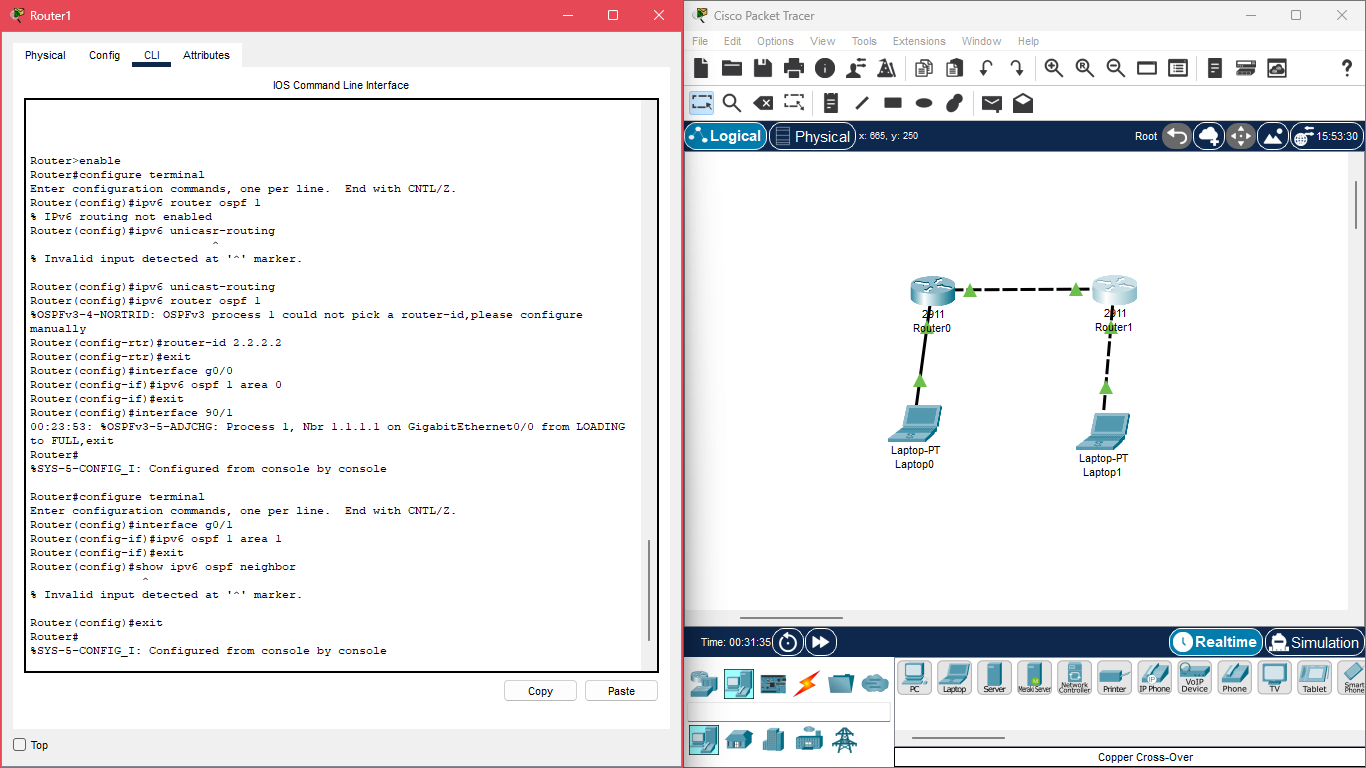
\includegraphics[width=0.5\textwidth]{tumod/jarkom tumod 2.png} 
    \caption{Setting OSPF di Router B} 
    \label{fig:tumod2} 
\end{figure}

\begin{figure}[H] 
    \centering
    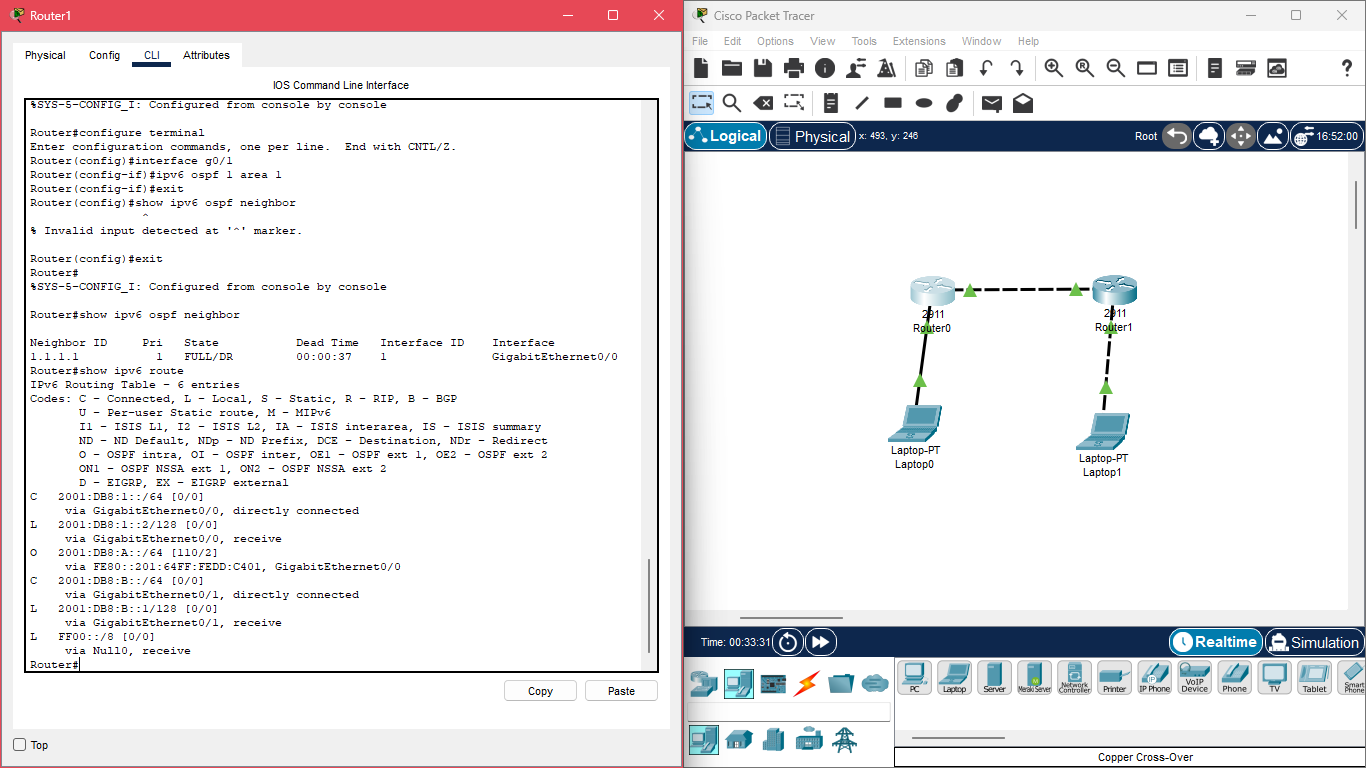
\includegraphics[width=0.5\textwidth]{tumod/jarkom tumod 4.png} 
    \caption{Setting OSPF di Router A} 
    \label{fig:tumod3} 
\end{figure}

\section{Kesimpulan}
Berdasarkan praktikum yang telah dilakukan, dapat diambil beberpaa kesimpulan penting. Yang pertama adalah penggunaan IPv6 yang mengutamakan kemudahan dimana pengguna tidak perlu memikirkan aspek penghematan alamat yang menjadi concern utama pada penggunaan IPv4. Selain itu, alamat IPv6 memiliki mekanisme penyingkatan yang efektif sehingga walaupun menyediakan wadah hingga 128 bit, penulisannya bisa tetap ringkas. Proses routing statis untuk IPv6 dan IPv4 tidak jauh berbeda. Begitu juga untuk routing dinamis, meskipun perlu diperhatikan dukungan IPv6 untuk versi protokolnya.

\section{Lampiran}
\subsection{Dokumentasi saat praktikum}

\begin{figure}[H] 
    \centering
    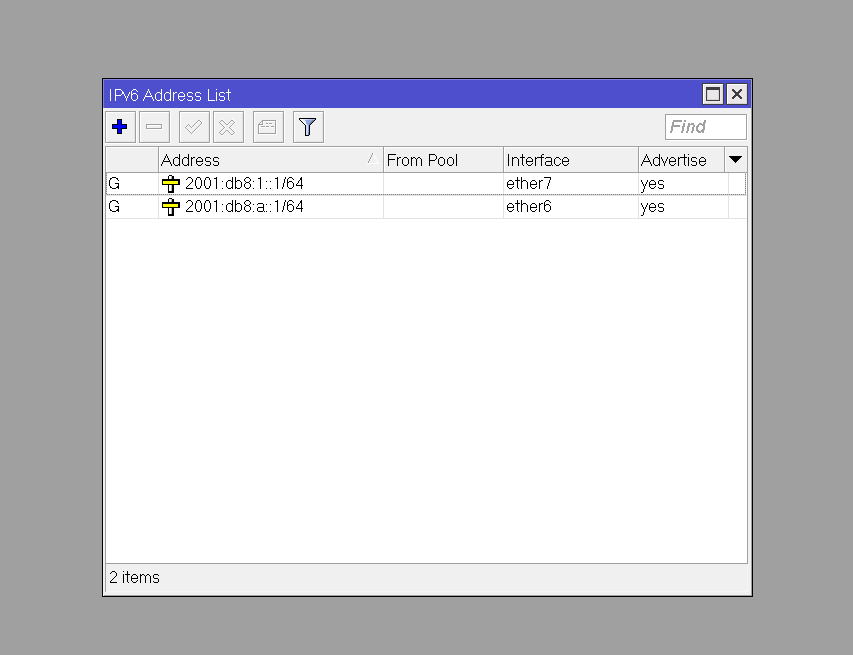
\includegraphics[width=0.5\textwidth]{Dokum P2/Laptop 1/assign ip.png} 
    \caption{Memberikan Alamat IPv6 ke Semua interfaces} 
    \label{fig:langkaha2} 
\end{figure}
\begin{figure}[H] 
    \centering
    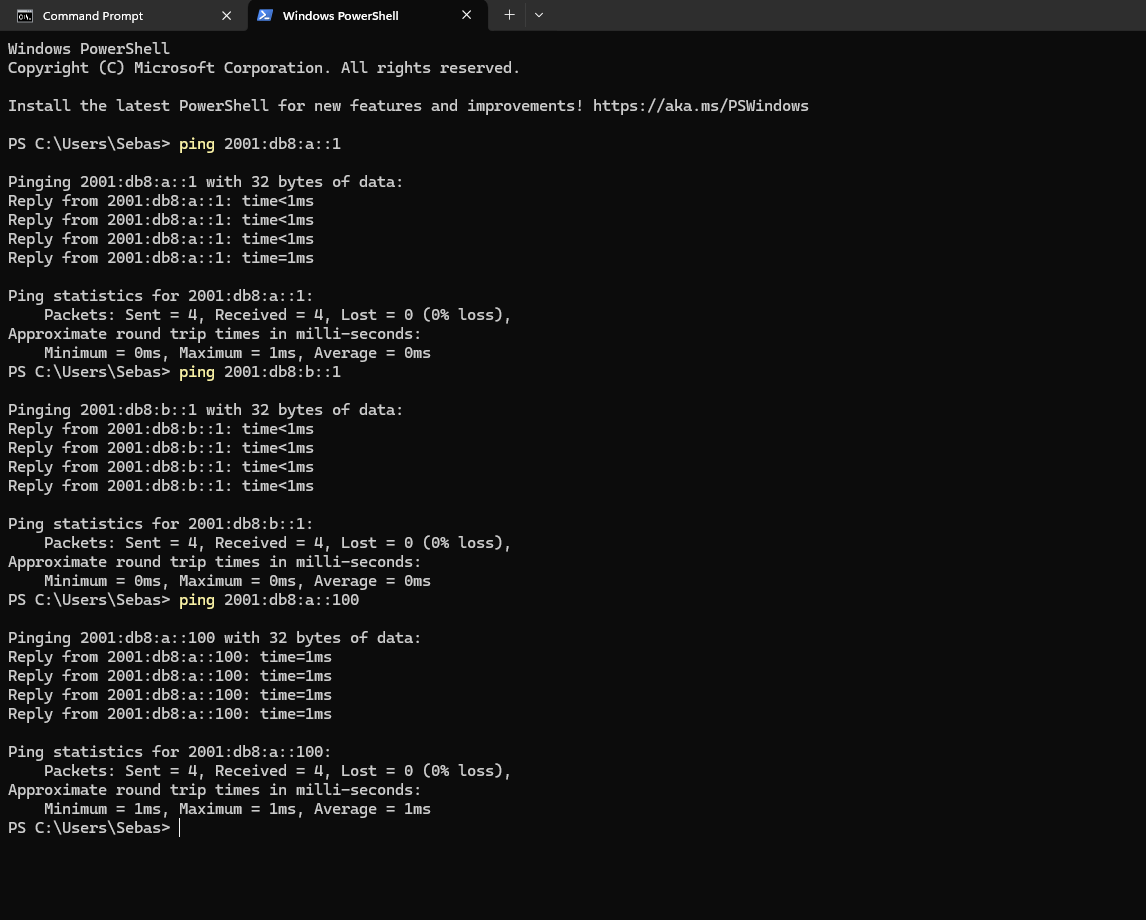
\includegraphics[width=0.5\textwidth]{Dokum P2/Laptop 2/ping laptop 1 ipv6.png} 
    \caption{Hasil Routing Table Statis} 
    \label{fig:langkaha5} 
\end{figure}
\begin{figure}[H] 
    \centering
    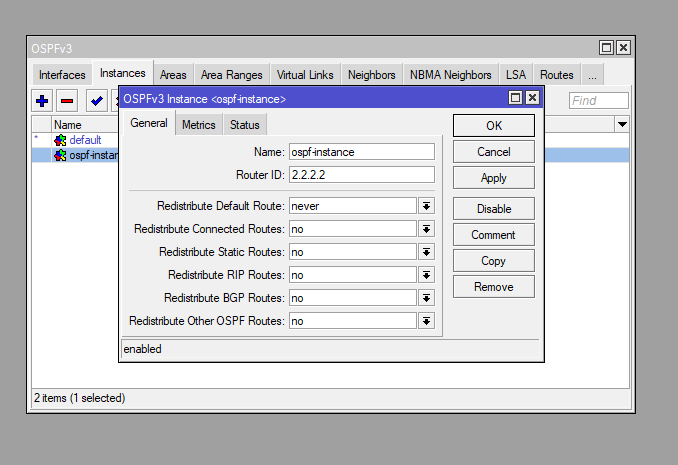
\includegraphics[width=0.5\textwidth]{Dokum P2/Laptop 2/jarkomp2-dinamis-instance-ospfv3.png} 
    \caption{Menyetel Instance OSPFv3} 
    \label{fig:langkahb2a} 
\end{figure}
\begin{figure}[H] 
    \centering
    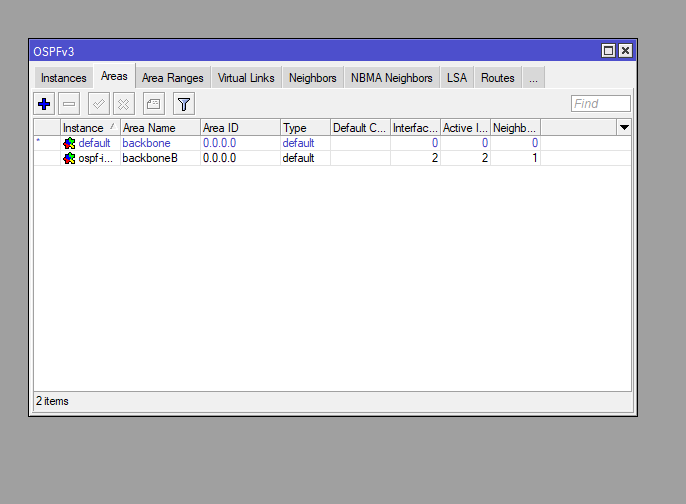
\includegraphics[width=0.5\textwidth]{Dokum P2/Laptop 2/jarkomp2-dinamis-2.png} 
    \caption{Menyetel Area OSPFv3} 
    \label{fig:langkahb2b} 
\end{figure}
\begin{figure}[H] 
    \centering
    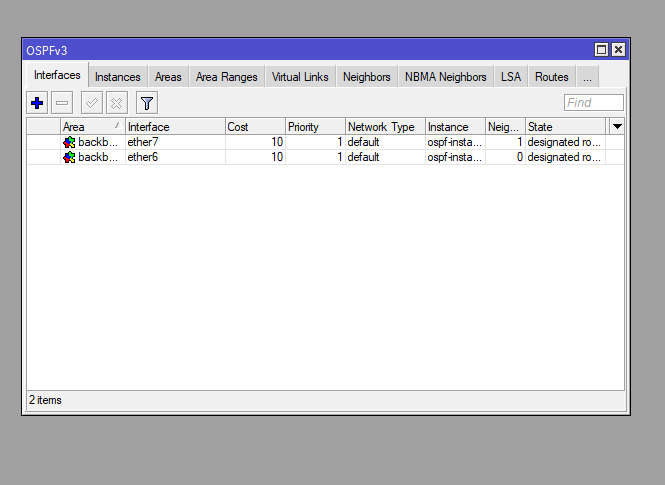
\includegraphics[width=0.5\textwidth]{Dokum P2/Laptop 2/jarkomp2-dinamis-3.png} 
    \caption{Menyetel Interface OSPFv3} 
    \label{fig:langkahb3} 
\end{figure}
\begin{figure}[H] 
    \centering
    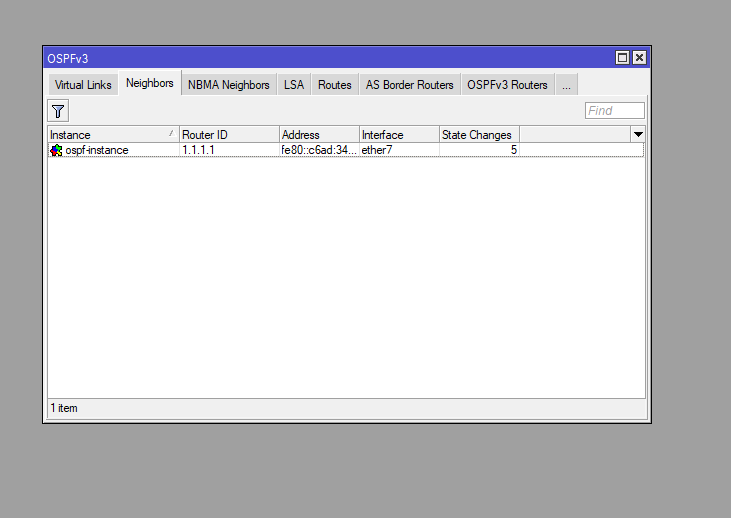
\includegraphics[width=0.5\textwidth]{Dokum P2/Laptop 2/jarkomp2-dinamis-4.png} 
    \caption{Melihat Neighbour OSPFv3} 
    \label{fig:langkahb4} 
\end{figure}
\begin{figure}[H] 
    \centering
    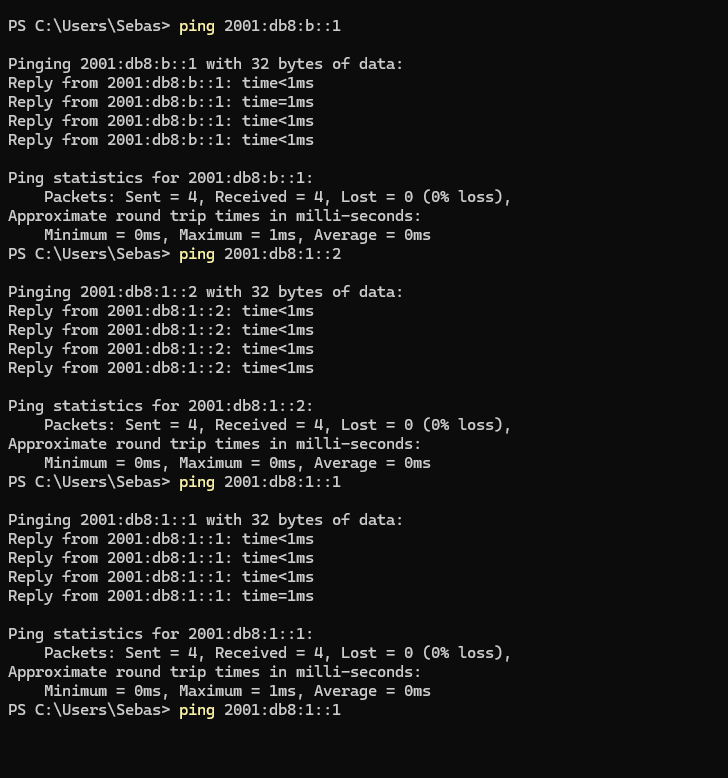
\includegraphics[width=0.5\textwidth]{Dokum P2/Laptop 2/jarkomp2-dinamis-5.png} 
    \caption{Menguji Konektivitas} 
    \label{fig:langkahb5} 
\end{figure}
\begin{figure}[H] 
    \centering
    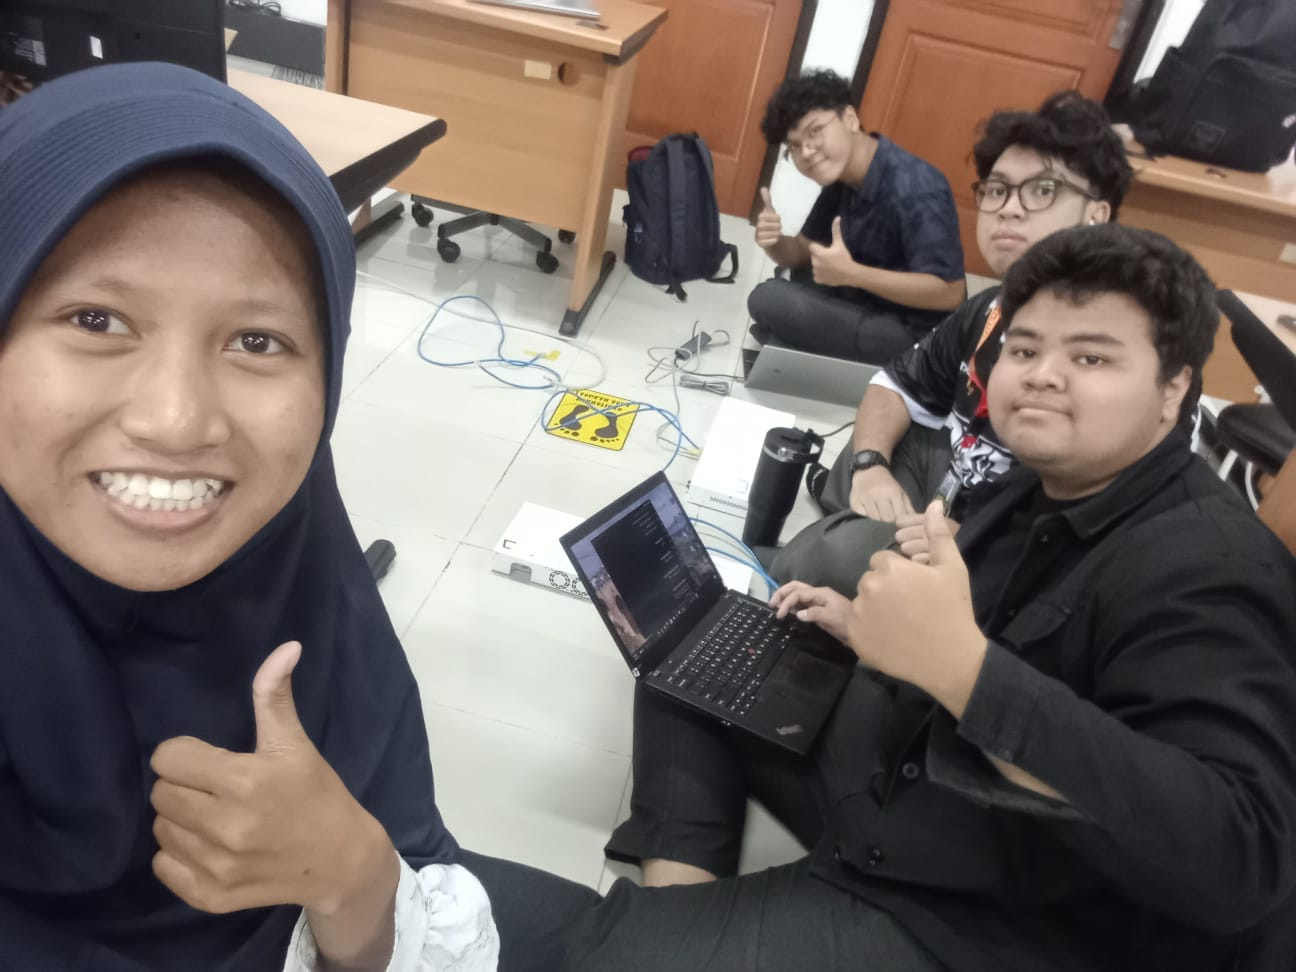
\includegraphics[width=0.5\textwidth]{Dokum P2/Dokum kelompok.jpg} 
    \caption{Dokumentasi Bersama Kelompok} 
    \label{fig:dokum} 
\end{figure}